% SPDX-License-Identifier: CC-BY-SA-4.0
% Author: Matthieu Perrin
% Part: 
% Section: 
% Sub-section: 
% Frame: 

\begingroup

\begin{frame}{Buts de la programmation multi-c\oe urs}

  \begin{exampleblock}{Calculs coûteux}
    \begin{itemize}
    \item En temps de processeur (simulations scientifiques, \dots)
    \item<2-> En entrées/sorties (recherche dans les fichiers, \dots)
    \end{itemize}
  \end{exampleblock}
  \uncover<3->{
    \begin{exampleblock}{Activités coopérantes}
      \begin{itemize}
      \item Interface réactive (compilation à la volée, \dots)
      \item Traitement de requêtes sur un serveur, \dots
      \end{itemize}
    \end{exampleblock}
    \begin{block}{Stratégie de parallélisation}
      \begin{itemize}
      \item Découper le problème en tâches indépendantes
      \item Associer des tâches à chaque c\oe ur 
      \item S'assurer que les c\oe urs collaborent correctement
      \end{itemize}
    \end{block}
  }

  \uncoverb<1>{
    \ob[y=-15mm]{
      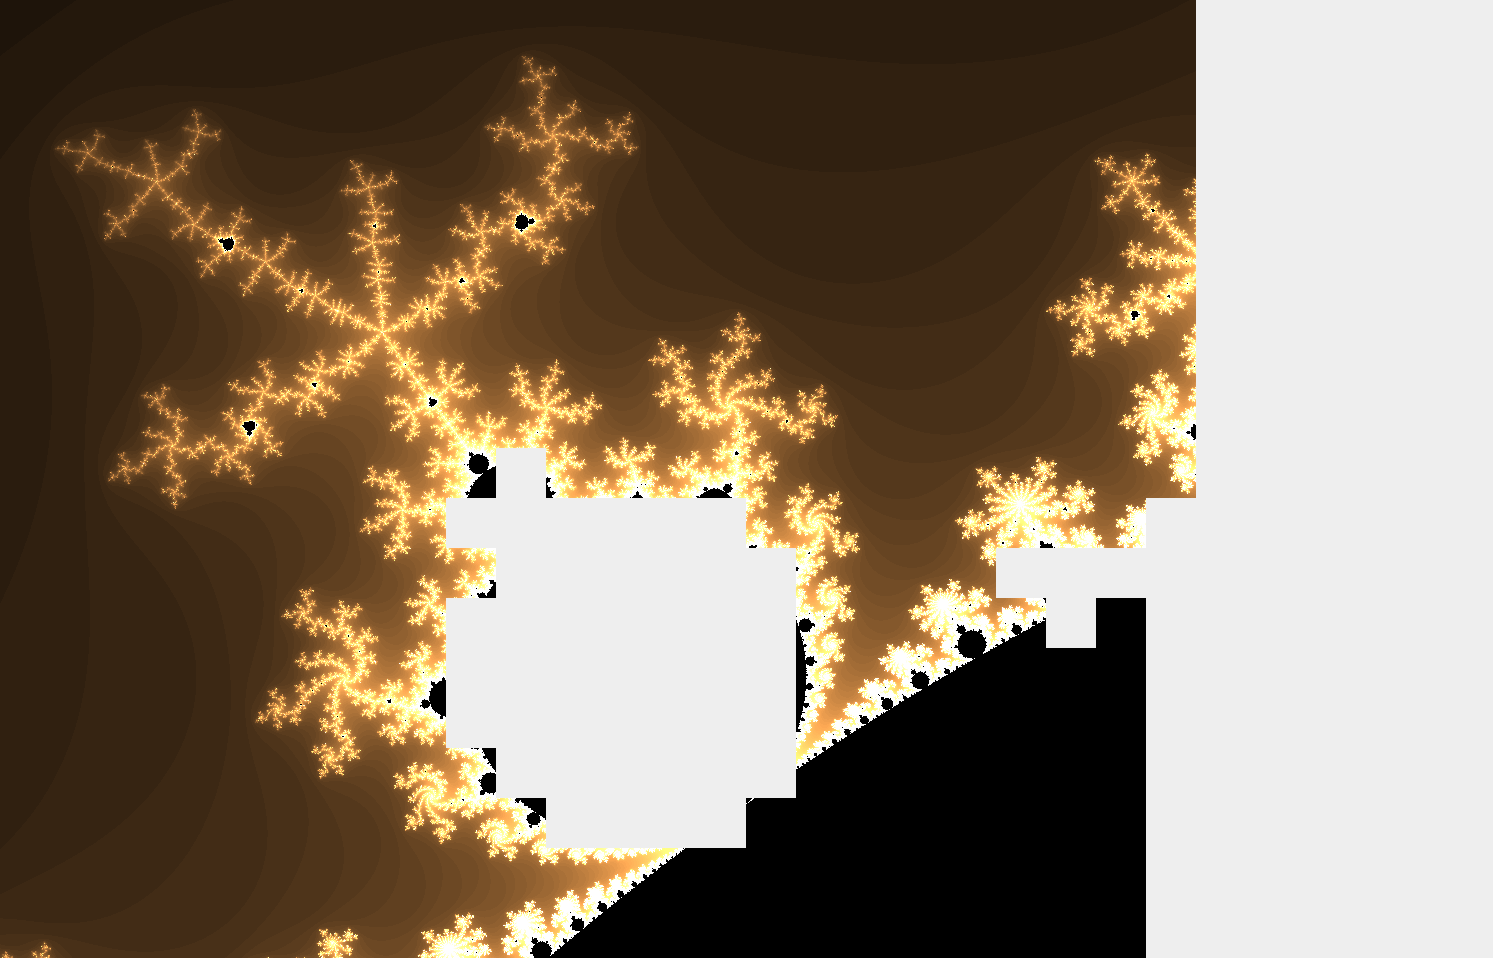
\includegraphics[height=.4\textwidth]{TP_Mandelbrot}
    }
  }

  \uncoverb<2>{
    \ob[y=-15mm]{
      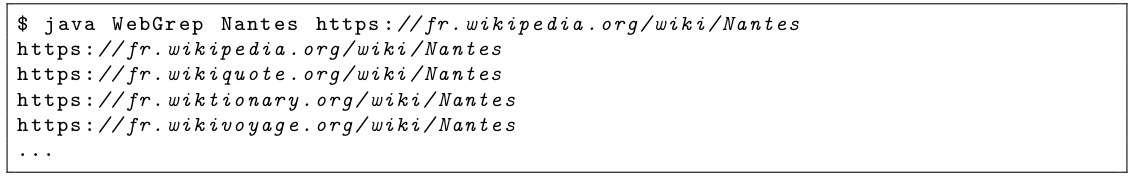
\includegraphics[width=.8\textwidth]{TP_WebGrep}
    }
  }

\end{frame}

\endgroup
\endinput
